%%%%%%%%%%%%%%%%%%%%%%%%%%%%%%%%%%%%%%%%%%%%%%%%%%%%%%%%%%%%%%%%%%%%%%%%%%%%%%%%%%%%%%%%%%%%%%%%%%%%
% 
% PRL presentation template
% based on https://github.com/FAU-AMMN/fau-beamer by Tim Roith
% Adaptation done by:
% Linda Schneider
% Dalia Rodriguez-Salas
% Noah Maul
%
% This program can be redistributed and/or modified under the terms
% of the GNU Public License, version 2.
%
%%%%%%%%%%%%%%%%%%%%%%%%%%%%%%%%%%%%%%%%%%%%%%%%%%%%%%%%%%%%%%%%%%%%%%%%%%%%%%%%%%%%%%%%%%%%%%%%%%%%

%\documentclass[handout, notes, t]{beamer}
%\documentclass[notes, t]{beamer}
\documentclass[t]{beamer}

\usepackage[utf8]{inputenc}
\usepackage[T1]{fontenc}


%%%%%%%%%%%%%%%%%%%%%%%%%%%%%%%%%%%%%%%%%%%%%%%%%%%%%%%%%%%%%%%%%%%%%%%%%%%%%%%%%%%%%%%%%%%%%%%%%%%%
%% STYLE
%%%%%%%%%%%%%%%%%%%%%%%%%%%%%%%%%%%%%%%%%%%%%%%%%%%%%%%%%%%%%%%%%%%%%%%%%%%%%%%%%%%%%%%%%%%%%%%%%%%%

% the possible options for the 'i2beamer' package are:
% - 'english' (if the slides are in english) 
% - 'wide'    (if the slides should use a 16:9 aspect ratio)
% - 'logo'    (if the logo of the Programming Systems Group should be included)
% - 'plain'   (if the background image of the title page should be omitted)
% - Faculty shorts: nat, phil, med, tf, rw, wiso, jura (no faculty short results in FAU)

\RequirePackage[wide,logo,tf,english]{sty/beamer}

%%%%%%%%%%%%%%%%%%%%%%%%%%%%%%%%%%%%%%%%%%%%%%%%%%%%%%%%%%%%%%%%%%%%%%%%%%%%%%%%%%%%%%%%%%%%%%%%%%%%
%% Bibliography
%%%%%%%%%%%%%%%%%%%%%%%%%%%%%%%%%%%%%%%%%%%%%%%%%%%%%%%%%%%%%%%%%%%%%%%%%%%%%%%%%%%%%%%%%%%%%%%%%%%%
\defbibheading{bibliography}{}
\addbibresource[label=primary]{references.bib}
\nocite{*}


% % % EIGENE BEFEHLE % % %
\newcommand{\Emph}[1]{\textbf{#1}}
\newcommand{\mynote}[1]{\note{\Huge{#1}}}
\newcommand{\spacy}{\texttt{spacy}}

\newcommand{\os}[1]{\onslide<+->{#1}}
\newcommand{\Os}[2]{\onslide<#1->{#2}}

\setbeamercovered{transparent=0}


%%%%%%%%%%%%%%%%%%%%%%%%%%%%%%%%%%%%%%%%%%%%%%%%%%%%%%%%%%%%%%%%%%%%%%%%%%%%%%%%%%%%%%%%%%%%%%%%%%%%
%% INFO
%%%%%%%%%%%%%%%%%%%%%%%%%%%%%%%%%%%%%%%%%%%%%%%%%%%%%%%%%%%%%%%%%%%%%%%%%%%%%%%%%%%%%%%%%%%%%%%%%%%%

\title{Modeling Hippocampus in context of language}
%\subtitle{Optional subtitle of document}

\author{Philipp Rost}
%\institute[Departmentname]{Friedrich-Alexander-Universität Erlangen-Nürnberg\\ Departmentname}
\institute{Friedrich-Alexander-Universität Erlangen-Nürnberg}

\date[Datum]{\today}

%%%%%%%%%%%%%%%%%%%%%%%%%%%%%%%%%%%%%%%%%%%%%%%%%%%%%%%%%%%%%%%%%%%%%%%%%%%%%%%%%%%%%%%%%%%%%%%%%%%%
%% DOCUMENT
%%%%%%%%%%%%%%%%%%%%%%%%%%%%%%%%%%%%%%%%%%%%%%%%%%%%%%%%%%%%%%%%%%%%%%%%%%%%%%%%%%%%%%%%%%%%%%%%%%%%

\begin{document}
	
% ======================================

\begin{frame}
	\titlepage
\end{frame}

\begin{frame}
	\frametitle{Agenda}
	
	\tableofcontents
\end{frame}

% ======================================

\section{Hippocampus}

\begin{frame}
	\frametitle{Hippocampus}
	\begin{itemize}
		\item<1-> Has the shape of a seahorse
		\item<2-> Key factor in forming memories (not preserving them!)
		\item<3-> Related to emotions
		\item<4-> Responsible for any kind of navigation (e.g. ranking stuff like danger of animals)
		\begin{itemize}
			\item<5-> Crafts a \Emph{cognitive room} of the ``surroundings'' by using \Emph{place cells} and \Emph{grid cells}
			\item<6-> Place cell: irregular arranged, fires at specific positions in space % [deutschlandfunk]
			\item<7-> Grid cell: lattice-like arranged, fires continuously
		\end{itemize}
	\end{itemize}
% --- BILDER -----------------------------------
	\begin{columns}
		% Spalte 1
		\begin{column}{0.5\textwidth}
			\begin{figure}
				\centering
					\includegraphics<6->[scale=1.0]{Bilder/Ortszelle_Beispiel.png}
				\Os{6}{
					\caption{Different colors represent different place cells (= states)}
				}	
			\end{figure}
		\end{column}
		% Spalte 2
		\begin{column}{0.5\textwidth}
			\begin{figure}
				\centering
					\includegraphics<7->[scale=0.18]{Bilder/Gitterzelle_Beispiel_2.png}
				\Os{7}{
					\caption{Grid cells can describes as triangulation}
				}		
			\end{figure}
		\end{column}
	\end{columns}
%\mynote{
\mynote{
	\begin{itemize}
		\item for classical navigational tasks we have ``place cells'' and ``grid cells''
		\item ``specific position'': snippet of pathway or in the staircase \\
		\item Beispiel für surroundings: These cells map pitches (Original: Orts- und Rasterzellen kartieren akustische Tonhöhen; deutschlandfunk-Artikel)
	\end{itemize}
	\bigskip
	Referenzen:
	\begin{itemize}
		\item Neue Erinnerungen formen: Pauls Masterarbeit
		\item Emotionen: Wikipedia-Artikel (dort stehen Quellen)
		\item Navigation: Steht sicher auch etwas bei Wikipedia, sonst PMA oder SR-Paper
	\end{itemize}
}
\end{frame}

% ======================================

\section{Successor Representation}

\begin{frame}
	\frametitle{Successor Representation}
	\begin{itemize}
		\item<1-> Claim: Hippocampus learns a map representing each state as a successor state which is encoded via place cell
		\begin{itemize}
		\Os{2}{
			\item Where does the claim originate?
		}
		\Os{3}{	
			The proposed technique works fine for spatial navigation.
		}
		\end{itemize}
		\item<4-> Mathematical principle roots in reinforcement learning (and transition probability matrices) and can be computed like
		\[
			M_a = \sum_{t=0}^{a}{ \gamma^tT^t }
%			M = \sum_{t=0}^{\infty}{ \gamma^tT^t } = (E_n - \gamma T)^{-1}
			\text{,}
		\]
		with discount factor $ \gamma \in (0, 1) $ and transition probability matrix $ T $ % and identity matrix $ E_n $.
		\item<5-> The policy is encoded in matrix $ T \Longrightarrow $ the SR is policy-dependent (it is based on RL)
		\item<6-> Row $ i $: resembles (all) successor states of state $ i $ (the higher the value the higher the chance to be in this state after the next step)
		\item<7-> Column $ j $: High value in component $ i $ means state $ j $ is visited regularly after starting at state $ i $
	\end{itemize}
\mynote{
	-- You can also calculate the SR up to infinity \\
	-- By $ \gamma $ you can control how influential further apart states are \\
	-- By multiplying $ T $ with itself $ n $-times you receive the probabilities of being in an arbitrary position after $ n $ steps. So, the SR is just a ``layerd'' transition probability matrix $ T $. \\
	-- Dadurch dass die vielen Übergangsmatrizen „übereinander“ gelegt werden, erhöhen sich die Werte in jedem Feld mit jedem Summanden. Ist ein Wert nun hoch, bedeutet das, man war „in vielen Zwischenständen“ dort. \\
}
\end{frame}

% ======================================

\begin{frame}
	\frametitle{Successor Representation}
	\framesubtitle{Example 1/2 of interpreting a SR matrix $ M $}
	\begin{figure}
	\centering
		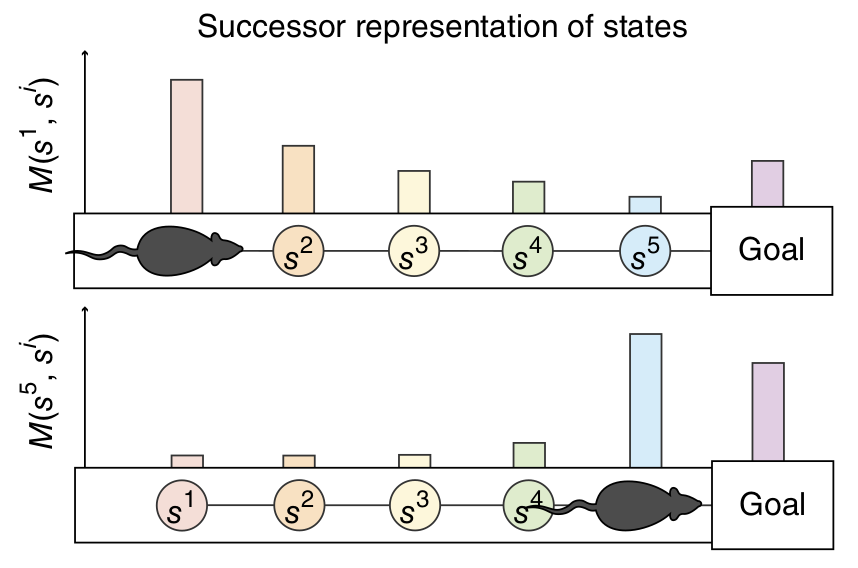
\includegraphics[scale=0.6]{Bilder/Beispiel_SR_Zeile.png}
	\end{figure}
	\notsoimportant{Superscript means index not power}
\mynote{
	-- 6 states \\
	-- Policy: going to right or staying in current location \\
	-- $ M(s^1, s') $ describes row of $ M $ and implies the following: Due to the ``stay or go to the right''-policy is the probability for the states $ s^1, \ s^2 $ the largest
}
\end{frame}

% ======================================

\begin{frame}
	\frametitle{Successor Representation}
	\framesubtitle{Example 2/2 of interpreting a SR matrix $ M $}
	\begin{figure}[c]
		\centering
			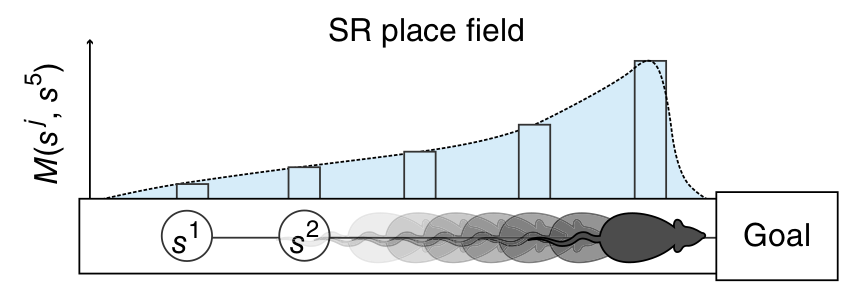
\includegraphics{Bilder/Beispiel_SR_Spalte.png}
	\end{figure}
\mynote{
	-- You can recognize the development of the policy: The more often the rat/mice goes to the right, the more likely it becomes reaching state $ s^4 $ or $ s^5 $ 
}
\end{frame}

% ======================================

\section{Goal of the thesis}
% TODO  meine Ansätze erläutern

% Diese Folie wird nach einem beispielhaftem Einschub auf einer weiteren fortgesetzt. Die Vollstände findet sich also auf der Übernächsten.
\begin{frame}
	\frametitle{Goal of the thesis}
	I try to answer: \emph{Does the Hippocampus, i.e. place (and grid) cells, generate a cognitive room of languages?} \\
	\bigskip
\Os{2}{
	Approach(es): Training a (shallow, supervised) neural network by...
	\smallskip
}
	\begin{enumerate}
		% TODO Fazit über die Güte der Funktionsweise direkt hier oder an anderer Stelle?
		\item<3-> building a graphical model based on word classes \label{enum: word classes}
		\begin{itemize}
			\item<4-> Word classes with made up rules like ``Pronoun $ \to $ Verb''
			\item<5-> Building a cognitive room: List of all words
			\item<6-> For each rule two 1 hot encoded vectors related to the cognitive room are used for training (first vector as input, second as preferable output)
			\item[$ \Rightarrow $]<7-> Works well due to graph environment 
%			\item<+-> For each rule a pair of word is generated
%			\item[$ \Rightarrow $]<+-> crafting a \Emph{1 hot encoded vector} associated to the cognitive room and used for training (first vector as input, second as preferable output)
		\end{itemize}
	\end{enumerate}
\mynote{
	-- \Emph{training data}: first word is input, second word is supervised output. So, the network should learn to predict the second one based on the primary word \\
	-- \Emph{1-hot-encoded vector}: Imagine having a list of all words, then we generate a 0-vector with equal length and note a 1 at the position of the word in the list. \\
	-- \Emph{word vectors}: For predicting/evaluation we invert the calculating of a word vector, which means receiving a word 
}
\end{frame}

% ======================================

\begin{frame}
	\frametitle{Example results for graphical model}
	Rules used: Question Word $ \to $ Personal Pronoun, Adjective $ \to $ Noun,	Personal Pronoun $ \to $ Verb \& Verb $ \to $ Adjective
	\begin{figure}[t]
		\centering
			\includegraphics[scale=0.35]{Bilder/SR + PCA_First Model_10E_50BS_1L_1C_2022.05.11-21:55:29}
	\end{figure}
\mynote{
	\begin{itemize}
		\item ``noun''-row smeary because no rule with first argument ``noun'' exists
		\item each color represents a word class
		\item clustering obvious $ \Longrightarrow $ Word classes recognizable
	\end{itemize}
}
\end{frame}


%\begin{frame}
%	\frametitle{Example}
%	\begin{columns}
%		% SPALTE 1
%		\begin{column}{0.3\textwidth}
%			Rules used:
%			\begin{itemize}
%				\item Question Word $ \to $ Personal Pronoun
%				\item Adjective $ \to $ Noun,
%				\item Personal Pronoun $ \to $ Verb
%				\item Verb $ \to $ Adjective
%			\end{itemize}
%		\end{column}
%	
%		% SPALTE 2
%		\begin{column}{0.7\textwidth}
%			\begin{figure}[!h]
%				\centering
%					\includegraphics[scale=0.35]{Bilder/SR + PCA_First Model_10E_50BS_1L_1C_2022.05.11-21:55:29}
%			\end{figure}
%		\end{column}
%	\end{columns}
%\end{frame}

% ======================================

\begin{frame}
	\frametitle{Goal of the thesis}
	We try to answer the question: \emph{Does the Hippocampus, i.e. place (and grid) cells, generate a cognitive map of languages?} \\
	\bigskip
	Approach(es): Training a (shallow, supervised) neural network by...
	\smallskip
	\begin{enumerate}
		% TODO Fazit über die Güte der Funktionsweise direkt hier oder an anderer Stelle?
		\item building a graphical model based on word classes
			\begin{itemize}
				\item Word classes with made up rules like ``Pronoun $ \to $ Verb''
				\item Building a cognitive room: List of all words
				\item For each rule two 1 hot encoded vectors related to the cognitive room are used for training (first vector as input, second as preferable output)
				%			\item<+-> For each rule a pair of word is generated
				%			\item[$ \Rightarrow $]<+-> crafting a \Emph{1 hot encoded vector} associated to the cognitive room and used for training (first vector as input, second as preferable output)
				\item[$ \Rightarrow $] Works well due to graph environment 
			\end{itemize}
		\item<2-> Parsing text to use two following words as training data by...
			\begin{itemize}
				\item<3-> Using 1 hot encoded vectors but without made up rules. Input \& output are determined by running order
				\item<4-> Calculating word vectors using \spacy % TODO Referenz hinzufügen
				\begin{itemize}
					\item<5-> \spacy \space can (bidirectionally) transfer between words and vectors
				\end{itemize}
				\item[$ \Rightarrow $]<6-> Works ...not really
			\end{itemize}
	\end{enumerate}
\os{
%	Technique \ref{enum: word classes} works well, because you can calculate transition matrices properly TODO \\ % TODO Warum genau? Wird wirklich ein Graph gelernt? Ich bin mir diesbezüglich gerade nicht mehr so sicher
%	Parsing texts in comparison not really TODO % TODO Paul fragen	
}
\mynote{
	-- \Emph{training data}: first word is input, second word is supervised output. So, the network should learn to predict the second one based on the primary word \\
	-- \Emph{1-hot-encoded vector}: Imagine having a list of all words, then we generate a 0-vector with equal length and note a 1 at the position of the word in the list. \\
	-- \Emph{word vectors}: For predicting/evaluation we invert the calculating of a word vector, which means receiving a word 
}
\end{frame}

% ======================================

\begin{frame}
	\frametitle{Example of word vector model}
	\begin{figure}[t]
		\centering
			\includegraphics[scale=0.35]{Bilder/Real Text spacy_concat_100E_100BS_10L_10C_2022.05.07-18:09:57.png}
	\end{figure}
\end{frame}

\end{document}